\subsubsection{Fabricación y ensamblado}

El diseño de hardware del SAL/T incluye algunos otros componentes no mencionados en los puntos anteriores. Las resistencias utilizadas en el proyecto son resistencias de película gruesa de montaje superficial (SMD), de 1/4 W, tolerancia del 1\% y tamaño 0805; se utilizaron los distintos valores que ofrece la empresa YAGEO para su serie RC. Para los capacitores se utilizaron generalmente capacitores cerámicos multicapa de KEMET, de montaje superficial tamaño 0805, tolerancia del 10\% y operan hasta 16 VDC. Para los capacitores electrolíticos, se utilizaron capacitores de aluminio de Panasonic de la serie HA con tolerancia 20\% y operación hasta 35 VDC. \\ 

En la tabla \ref{tab:bom}, se visualiza el listado completo de los componentes (BOM) necesarios para fabricar el prototipo del SAL/T con sus precios en dólares estadounidenses expuestos por el distribuidor Mouser Electronics que suma un total de 362.97 USD: 

\begin{table}[H]
\begin{tabular}{|c|c|c|c|c|c|}
 \hline
 & Fabricante          & Modelo                                                                                                                                                                                                                                    & Cantidad & Precio & Precio \\ 
 
 &           &                                                                                                                                                                                                                                     &  & unitario & del item \\ 
 \hline
1                    & KEMET               & \href{https://ar.mouser.com/datasheet/2/447/KEM_C1002_X7R_SMD-3316098.pdf}{C1206C106K4RACTU}                                                                                                                        & 5        & 0,35            & 1,75            \\ \hline
2                    & KEMET               & \href{https://ar.mouser.com/datasheet/2/447/KEM_C1002_X7R_SMD-3316098.pdf}{C0805C104K4RACTU}                                                                                                                        & 25       & 0,14            & 3,50            \\ \hline
3                    & Panasonic           & \href{http://industrial.panasonic.com/cdbs/www-data/pdf/RDE0000/ABA0000C1148.pdf}{EEE-HAV100WAR}                                                                                                                       & 3        & 0,38            & 1,13            \\ \hline
4                    & LITTELFUSE          & \href{https://www.littelfuse.com/$\sim$/media/electronics/datasheets/tvs_diodes/littelfuse_tvs_diode_szp6smb_datasheet.pdf.pdf}{SZP6SMB12CAT3G}                                                                   & 6        & 0,43            & 2,58            \\ \hline
5                    & Wurth Elektronik    & \href{https://www.we-online.com/catalog/datasheet/150080VS75000.pdf}{150080VS75000}                                                                                                                                    & 22       & 0,19            & 4,11            \\ \hline
6                    & Lite-On             & \href{https://componentsearchengine.com/Datasheets/1/LTC-5723HR.pdf}{LTC-5723HR}                                                                                                                                       & 1        & 2,99            & 2,99            \\ \hline
7                    & Bourns              & \href{https://www.bourns.com/docs/Product-Datasheets/mfusmf.pdf}{MF-USMF020-2}                                                                                                                                         & 4        & 0,34            & 1,36            \\ \hline
8                    & Vishay              & \href{https://www.vishay.com/docs/72079/si2343ds.pdf}{SI2343DS-T1-E3}                                                                                                                                                  & 1        & 0,75            & 0,75            \\ \hline
9                    & STMicroelectronics  & \href{http://www.st.com/st-web-ui/static/active/en/resource/technical/document/datasheet/CD00001244.pdf}{ULN2003D1013TR}                                                                                               & 4        & 0,73            & 2,91            \\ \hline
10                   & Texas Instruments   & \href{https://www.ti.com/lit/ds/symlink/ina823.pdf}{INA823DGKR}                                                                                                                                                        & 10       & 2,35            & 23,50           \\ \hline
11                   & Renesas Electronics & \href{https://www.renesas.com/en-us/www/doc/datasheet/icl7660s-a.pdf}{ICL7660AIBAZA}                                                                                                                                   & 1        & 2,03            & 2,03            \\ \hline
12                   & ams                 & \href{https://datasheet.datasheetarchive.com/originals/distributors/Datasheets-SFU1/DSASFU10002655.pdf}{AS1115-BSST}                                                                                                   & 1        & 6,58            & 6,58            \\ \hline
13                   & Phoenix Contact     & \href{http://www.phoenixcontact.com/de/produkte/1757491/pdf}{1757491}                                                                                                                                                  & 8        & 1,32            & 10,56           \\ \hline
14                   & Phoenix Contact     & \href{http://www.phoenixcontact.com/de/produkte/1757488/pdf}{1757488}                                                                                                                                                  & 11       & 1,06            & 11,66           \\ \hline
15                   & Amphenol FCI        & \href{https://ar.mouser.com/datasheet/2/18/1/87583-2579162.pdf}{87583-2010BLF}                                                                                                                                         & 2        & 1,07            & 2,14            \\ \hline
16                   & Hirose              & \href{https://datasheet.lcsc.com/szlcsc/Hirose-HRS-DM3AT-SF-PEJM5_C114218.pdf}{DM3AT-SF-PEJM5}                                                                                                                        & 1        & 2,63            & 2,63            \\ \hline
17                   & Phoenix Contact     & \href{http://www.phoenixcontact.com/de/produkte/1757475/pdf}{1757475}                                                                                                                                                  & 1        & 0,73            & 0,73            \\ \hline
18                   & SparkFun            & \href{https://cdn.sparkfun.com/assets/1/c/f/7/9/DS-16581-Female_Header_2x18.pdf}{PRT-09044}                                                                                                                          & 8        & 0,38            & 3,04            \\ \hline
19                   & Panasonic           & \href{https://www3.panasonic.biz/ac/e_download/control/relay/power/catalog/mech_eng_jw.pdf}{JW2SN-DC5V}                                                                                                             & 21       & 2,10            & 44,10           \\ \hline
20                   & Kingbright          & \href{https://www.mouser.com/datasheet/2/216/WP7113LZGCK-535810.pdf}{WP7113LZGCK}                                                                                                                                      & 8        & 0,36            & 2,89            \\ \hline
21                   & Kingbright          & \href{http://www.kingbrightusa.com/images/catalog/SPEC/WP154A4SEJ3VBDZGW-CA.pdf}{WP154A4SEJ3VBDZGW/CA}                                                                                                                 & 10       & 1,36            & 13,60           \\ \hline
22                   & CUI Devices         & \href{https://www.cuidevices.com/product/resource/cem-1205-ic.pdf}{CEM-1205-IC}                                                                                                                                        & 1        & 1,91            & 1,91            \\ \hline
23                   & onsemi              & \href{https://componentsearchengine.com/Datasheets/2/NVTR0202PLT1G.pdf}{NVTR0202PLT1G}                                                                                                                                 & 1        & 0,38            & 0,38            \\ \hline
24                   & YAGEO               & \href{https://ar.mouser.com/datasheet/2/447/PYu_RC_Group_51_RoHS_L_11-1984063.pdf}{RC0805FR-104K7L}                                                                                                              & 6        & 0,10            & 0,60            \\ \hline
25                   & YAGEO               & \href{https://ar.mouser.com/datasheet/2/447/YAGEO_PYu_RC_Group_51_RoHS_L_12-3313492.pdf}{RC0805FR-10100KL}                                                                                                      & 4        & 0,10            & 0,40            \\ \hline
26                   & YAGEO               & \href{https://ar.mouser.com/datasheet/2/447/YAGEO_PYu_RC_Group_51_RoHS_L_12-3313492.pdf}{RC0805FR-07390RL}                                                                                                      & 4        & 0,10            & 0,40            \\ \hline
27                   & YAGEO               & \href{https://ar.mouser.com/datasheet/2/447/PYu_RC_Group_51_RoHS_L_11-1984063.pdf}{RC0805FR-13220RL}                                                                                                             & 2        & 0,10            & 0,20            \\ \hline
28                   & YAGEO               & \href{https://ar.mouser.com/datasheet/2/447/PYu_RC_Group_51_RoHS_L_11-1984063.pdf}{RC0805FR-10100RL}                                                                                                             & 3        & 0,02            & 0,05            \\ \hline
29                   & YAGEO               & \href{https://ar.mouser.com/datasheet/2/447/PYu_RC_Group_51_RoHS_L_11-1984063.pdf}{RC0805FR-13150KL}                                                                                                             & 2        & 0,10            & 0,20            \\ \hline
30                   & YAGEO               & \href{https://ar.mouser.com/datasheet/2/447/PYu_RC_Group_51_RoHS_L_11-1984063.pdf}{RC0805FR-13680RL}                                                                                                             & 22       & 0,10            & 2,20            \\ \hline
31                   & YAGEO               & \href{https://ar.mouser.com/datasheet/2/447/YAGEO_PYu_RC_Group_51_RoHS_L_12-3313492.pdf}{RC0805FR-0740K2L}                                                                                                      & 5        & 0,10            & 0,50            \\ \hline
32                   & YAGEO               & \href{https://ar.mouser.com/datasheet/2/447/PYu_RC_Group_51_RoHS_L_11-1984063.pdf}{RC0805FR-1056KL}                                                                                                              & 3        & 0,10            & 0,30            \\ \hline
33                   & YAGEO               & \href{https://ar.mouser.com/datasheet/2/447/PYu_RC_Group_51_RoHS_L_11-1984063.pdf}{RC0805FR-101ML}                                                                                                               & 20       & 0,10            & 2,00            \\ \hline
34                   & YAGEO               & \href{https://ar.mouser.com/datasheet/2/447/YAGEO_PYu_RC_Group_51_RoHS_L_12-3313492.pdf}{RC0805FR-0730KL}                                                                                                       & 20       & 0,10            & 2,00            \\ \hline
35                   & YAGEO               & \href{https://ar.mouser.com/datasheet/2/447/PYu_RC_Group_51_RoHS_L_11-1984063.pdf}{RC0805FR-1022KL}                                                                                                              & 2        & 0,10            & 0,20            \\ \hline
36                   & Bourns              & \href{https://www.arrow.com/en/products/1543-650-149/bourns}{1543-650-149}                                                                                                                                             & 1        & 1,21            & 1,21            \\ \hline
37                   & STMicroelectronics  & \href{https://ar.mouser.com/datasheet/2/389/nucleo_l496zg-1848160.pdf}{NUCLEO-F429ZI}                                                                                                                                 & 1        & 24,47           & 24,47           \\ \hline
38                   & Texas Instruments   & \href{http://www.ti.com/lit/gpn/sn65hvd1176}{SN65HVD1176DR}                                                                                                                                                            & 2        & 2,94            & 5,88            \\ \hline
39                   & u-Blox              & \href{https://www.datasheethub.com/gy-neo6mv2-flight-control-gps-module/}{GPS GY-NEO6MV2}                                                                                                                              & 1        & 13,48           & 13,48           \\ \hline
40                   & Espressif Systems   & \href{https://docs.espressif.com/projects/esp-idf/en/latest/esp32/hw-reference/esp32/get-started-devkitc.html}{ESP32-DevKitC-32E}                                                                                      & 1        & 13,87           & 13,87           \\ \hline
41                   & Harwin              & \href{https://ar.mouser.com/datasheet/2/181/M20-977-1220590.pdf}{M20-9774046}                                                                                                                                          & 6        & 1,47            & 8,82            \\ \hline
42                   & Elibet              & \href{https://articulo.mercadolibre.com.ar/MLA-715063582-llave-interruptor-bipolar-20a-elibet-0-1-panel-_JM\#position=4\&search_layout=stack\&type=item\&tracking_id=a983e77f-e6e3-4bab-bc34-8ba853ec8955}{20002/0} & 2        & 10,60           & 21,20           \\ \hline
43                   & Altanet             & \href{https://www.voipexperts.com.ar/index.php?option=com_k2\&Itemid=136\&id=953_bc11baf33c1825b2df10adc8c4f9a628\&lang=es\&task=download\&view=item}{AltaNet Stick ST10 4G WiFi}                                    & 2        & 44,77           & 89,54           \\ \hline
44                   & Phoenix Contact     & \href{https://www.phoenixcontact.com/us/products/1934887/pdf}{1934887}                                                                                                                                                 & 8        & 1,00            & 7,96            \\ \hline
45                   & Phoenix Contact     & \href{https://www.phoenixcontact.com/us/products/1935022/pdf}{1935022}                                                                                                                                                 & 11       & 0,71            & 7,77            \\ \hline
46                   & Phoenix Contact     & \href{https://www.phoenixcontact.com/us/products/1934861/pdf}{1934861}                                                                                                                                                 & 1        & 0,55            & 0,55            \\ \hline
47                   & Samtex              & \href{https://www.mouser.fr/datasheet/2/527/ssw_th-2854740.pdf}{SSW-119-01-T-S}                                                                                                                                       & 2        & 2,44            & 4,88            \\ \hline
48                   & Adam Tech           & \href{https://www.mouser.fr/datasheet/2/4/rs1_xx_g_data_sheet-3396051.pdf}{RS1-04-G}                                                                                                                               & 1        & 0,23            & 0,23            \\ \hline
49                   & SparkFun            & \href{https://www.mouser.fr/ProductDetail/SparkFun/PRT-16581?qs=sPbYRqrBIVmf2mq2gyI4eA\%3D\%3D}{PRT-16581}                                                                                                             & 4        & 1,81            & 7,24       \\ \hline

\end{tabular}
\caption{Listado de componentes del SAL/T}
\label{tab:bom}
\end{table}



Con el listado de materiales y sus hojas de datos presentes (que pueden ser accedidas mediante el hipervínculo colocado sobre cada modelo de componente en la tabla \ref{tab:bom}), se calculó el consumo máximo de potencia del SAL/T. La potencia total máxima que puede consumir el sistema, considerando que todos los componentes están trabajando al máximo de consumo lo que es un caso improbable, es de 18.38 W. El principal componente de la potencia son los relés que individualmente consumen 106mA cada uno al estar activados y hay 21 relés en todo el sistema. Los módulos USB Wi-Fi-4G, considerados para el cálculo de potencia, también tienen un gran consumo de 500mA cada uno, ya que necesitar generar la señal de la red Wi-Fi. Los módulos de GPS, ESP32 y Nucleo consumen alrededor de 100mA cada uno. El resto de los componentes suman de manera insignificante al número total. Por eso, se considera necesario una fuente de 5V con potencia de 20W para alimentar el SAL/T. \\


El diseño del sistema considera para todos los circuitos integrados un capacitor de 100nF de desacople para conectar cerca de su pin de alimentación entre VCC y tierra con el objetivo de filtrar ruidos que puedan estar presentes en la línea de alimentación. Para los casos más sensibles, también se contempló un capacitor electrolítico de 10 $\mu$F con la idea de reforzar el filtrado para ruidos de distintas frecuencias. También, en los esquemáticos se colocó una resistencia de 0 $\Omega$ al previo a conectar la línea de alimentación con el pin VCC de los chips para permitir el armado progresivo y segmentado del circuito una vez fabricado.  La selección de componentes consideró utilizar la menor cantidad posible de componentes \textit{through-hole} priorizando los de montaje superficial porque en aplicaciones ferroviarias, los componentes \textit{through-hole} pueden sufrir cortes o daños por las vibraciones de la formación.\\

Para conectar los módulos a la placa, se eligió utilizar conectores hembra tipo zócalo soldados a la placa para permitir colocar y sacar los módulos de manera más simple para su manipulación, programación y eventual reemplazo. Para la conexión con los sistemas externos, se utilizaron conectores de tipo bornera con tornillo soldados a la placa que permiten la conexión de cables. El sistema cuenta con 20 borneras en total y es por eso que cada una tiene identificada su función así como cada pin tiene indicada a qué señal corresponde. Esto aplica también para todos los componentes del sistema que tienen señalado qué número de componente corresponde a cada \textit{footprint} para facilitar el armado y el mantenimiento de las placas ante cualquier inconveniente. También se colocaron puntos de prueba en la mayoría de las señales relevantes para el sistema para poder medir el estado eléctrico de cada señal durante el armado, \textit{debugging} y pruebas del sistema. \\



Se intentó utilizar anchos de pista grandes para evitar quiebres en las pistas por vibraciones o flexiones de la placa y reducir la resistencia de las pistas también fue necesario utilizar distintos anchos para poder realizar el ruteo entre pines de la placa Núcleo. Se utilizaron anchos de .3mm, .4mm, .5mm y .8mm considerando el mayor ancho para las señales de alimentación o que transportan mayor corriente. Las vías se hicieron de 1mm con agujero de .4mm. Para los conectores de las borneras, se siguió la recomendación de utilizar agujeros grandes de 3mm/1.4mm y pistas anchas de .8mm para reducir el daño que pueda causar las fricciones provocadas por el procedimiento de instalación utilizando los tornillos de la bornera. Los puntos de prueba se hicieron de 1.53mm/1.02 para permitir utilizar la punta de un tester común para medir las señales. Además, las placas cuentan con agujeros para el montaje de la placa en el gabinete que se hicieron siguiendo el formato de tornillo M3 de diámetro 3.2mm. \\

En la tabla \ref{tab:design_constraints} se visualizan algunas de las restricciones utilizadas como reglas de diseño:

\begin{table}[H]
    \centering
    \begin{tabular}{|c|c|}
        \hline
         \textbf{Restricción} & \textbf{Valor}  \\ \hline
         Cobre - mínima distancia entre pistas & 0.2mm  \\ \hline
         Cobre - mínimo ancho de pista & 0.3mm  \\ \hline
         Cobre - mínimo ancho anular  & 0.25mm  \\ \hline
         Cobre - mínimo diámetro de vía  & 1mm  \\ \hline
         \textit{Holes} - mínimo diámetro del agujero & 0.3mm \\ \hline
         \textit{Holes} - mínimo distancia entre agujeros & 0.254mm \\
         \hline
    \end{tabular}
    \caption{Restricciones de diseño utilizadas para el diseño del PCB}
    \label{tab:design_constraints}
\end{table}


En ambas placas, se utilizó una de las capas como plano de tierra intentando utilizar la menor cantidad de pistas por ese lado mientras que la otra capa se utilizó para hacer todas las conexiones posibles. En las figuras \ref{fig:salt_tracks} y \ref{fig:salt_ihm_tracks} se visualiza los trazos de las pistas diseñados en ambas placas: 


\begin{figure}[H]
    \centering
    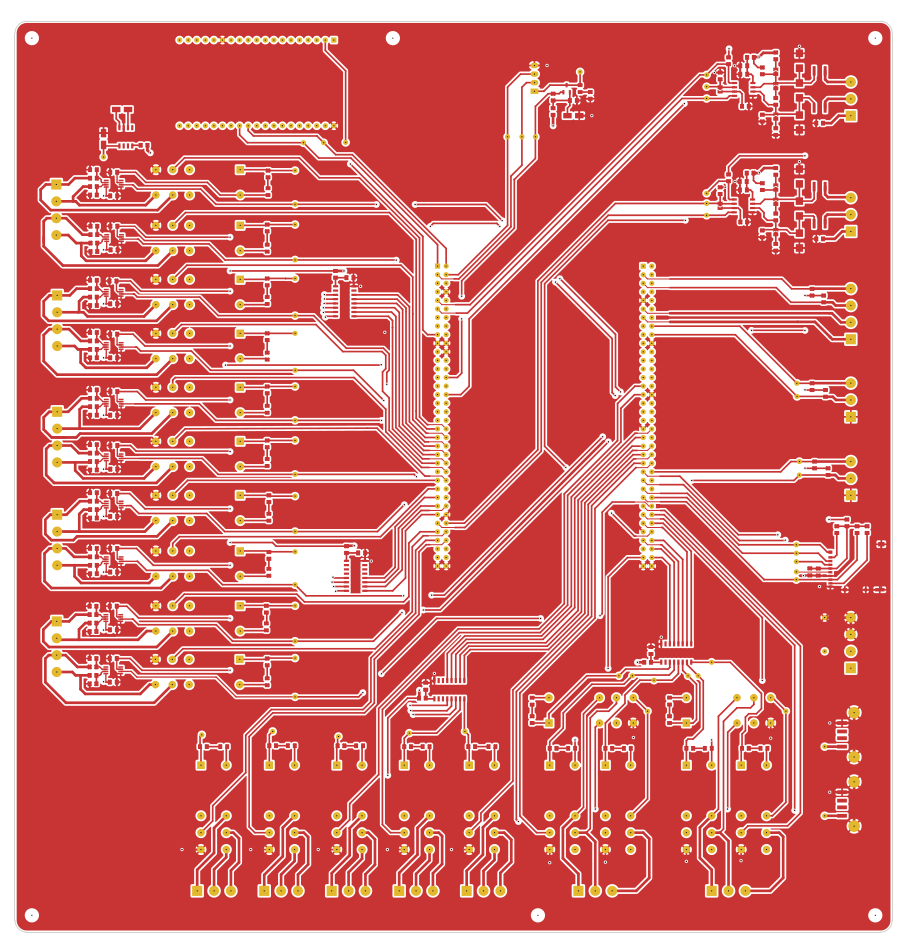
\includegraphics[width = 0.49\linewidth]{img/salt_tracks_front.png}
    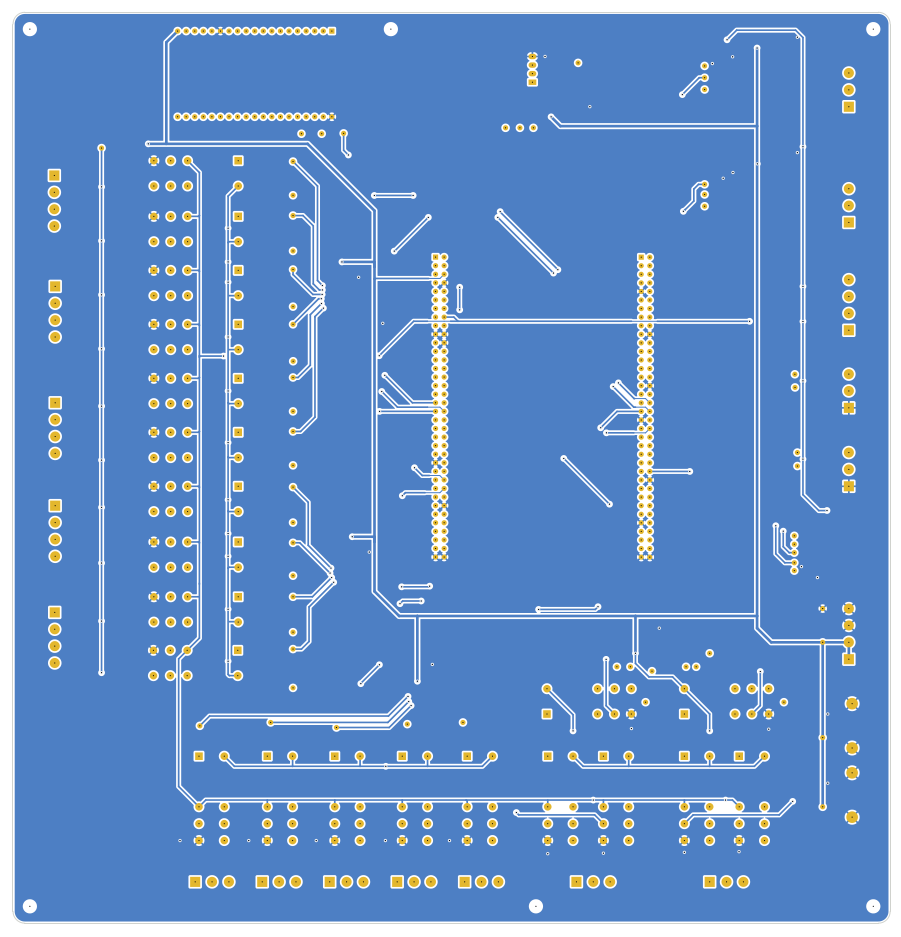
\includegraphics[width = 0.49\linewidth]{img/salt_tracks_back.png}
    \caption{Pistas y planos de la placa principal del SAL/T}
    \label{fig:salt_tracks}
\end{figure}    

\begin{figure}[H]
    \centering
    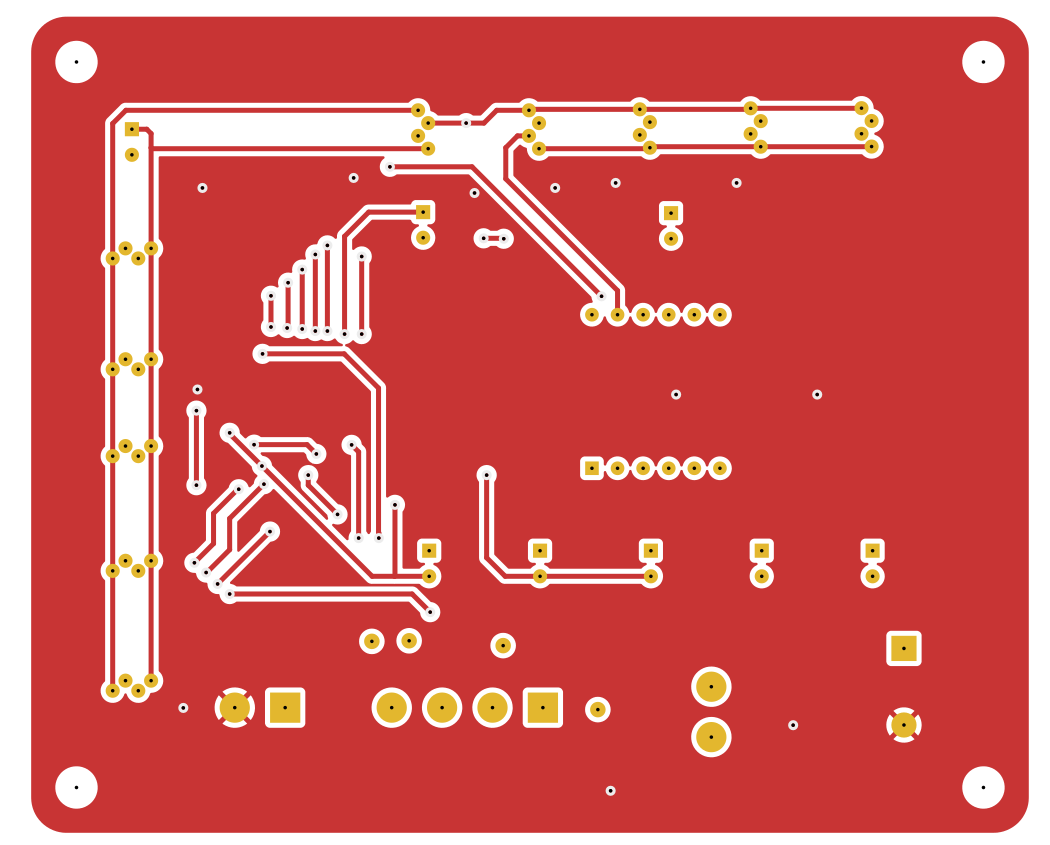
\includegraphics[width = 0.49\linewidth]{img/salt_ihm_tracks_front.png}
    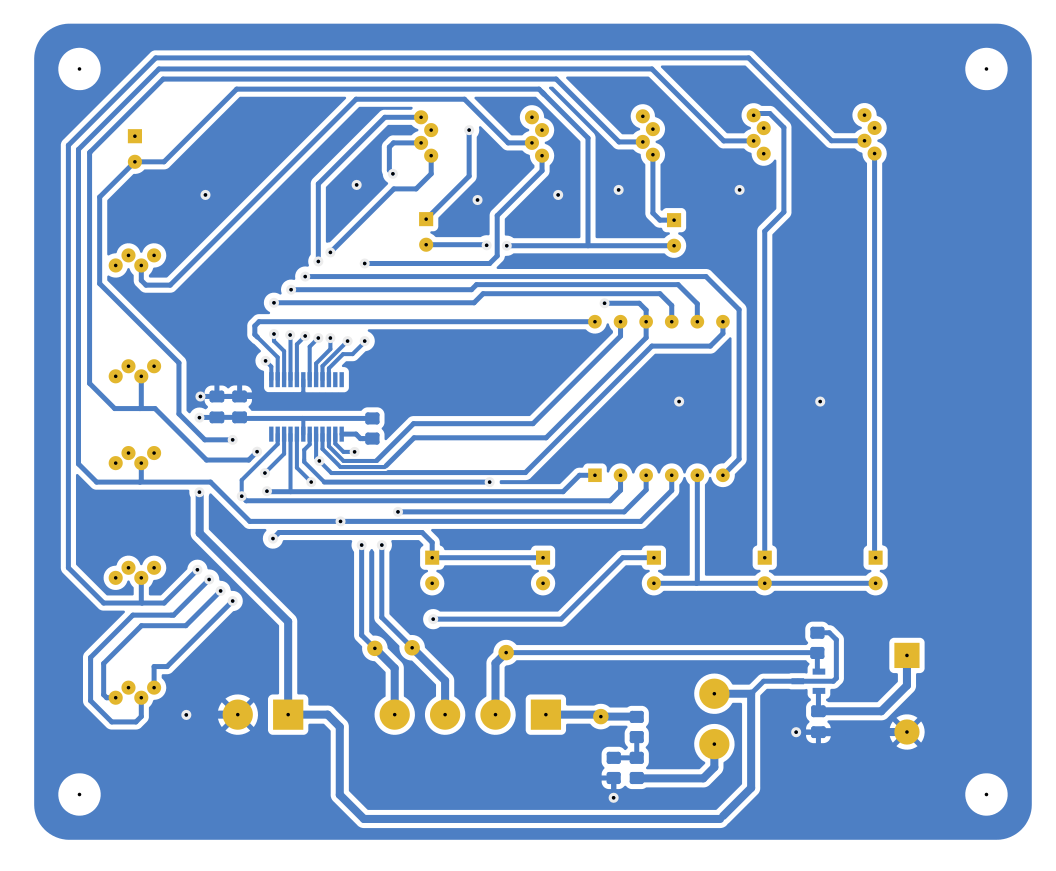
\includegraphics[width = 0.49\linewidth]{img/salt_ihm_tracks_back.png}
    \caption{Pistas y planos de la placa secundaria del SAL/T}
    \label{fig:salt_ihm_tracks}
\end{figure}    



Respecto al PCB (\textit{Printed Circuit Board}), se mandó a fabricar con la empresa JLCWAY \cite{jlcway} en China. Se utilizó el material FR-4, compuesto de fibra de vidrio y resina epoxi, para el substrato por su aislamiento eléctrico, su resistencia térmica y la relación entre rendimiento y costo lo que lo hace el estándar de la industria de PCBs. Ambas placas se fabricaron con 2 capas, la principal con dimensiones de 270mm x 260 mm mientras que la placa secundaria utilizada para el panel frontal mide 82mm x 100 mm. Se utilizó un grosor de placa de 1.6mm, placas de color verde con el \textit{silkscreen} (capa de serigrafía que contiene textos y símbolos impresos sobre la placa para identificar componentes, pines, y otras marcas importantes durante la fabricación y ensamblaje) de color blanco. En las figuras \ref{fig:salt_3d} y \ref{fig:salt_ihm_3d} se visualizan los modelos 3D de las placas diseñadas: 

\begin{figure}[H]
    \centering
    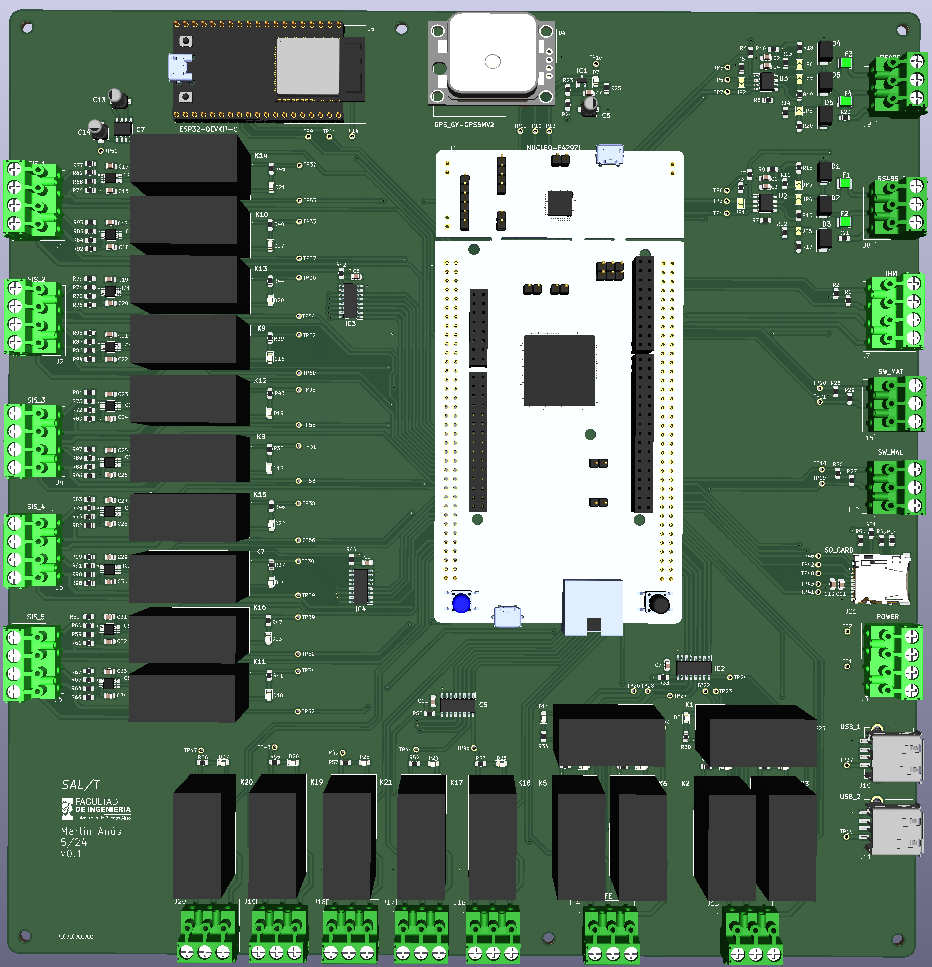
\includegraphics[width = \linewidth]{img/pcb_3d.png}
    \caption{Modelo 3D de la placa principal del SAL/T}
    \label{fig:salt_3d}
\end{figure}    



\begin{figure}[H]
    \centering
    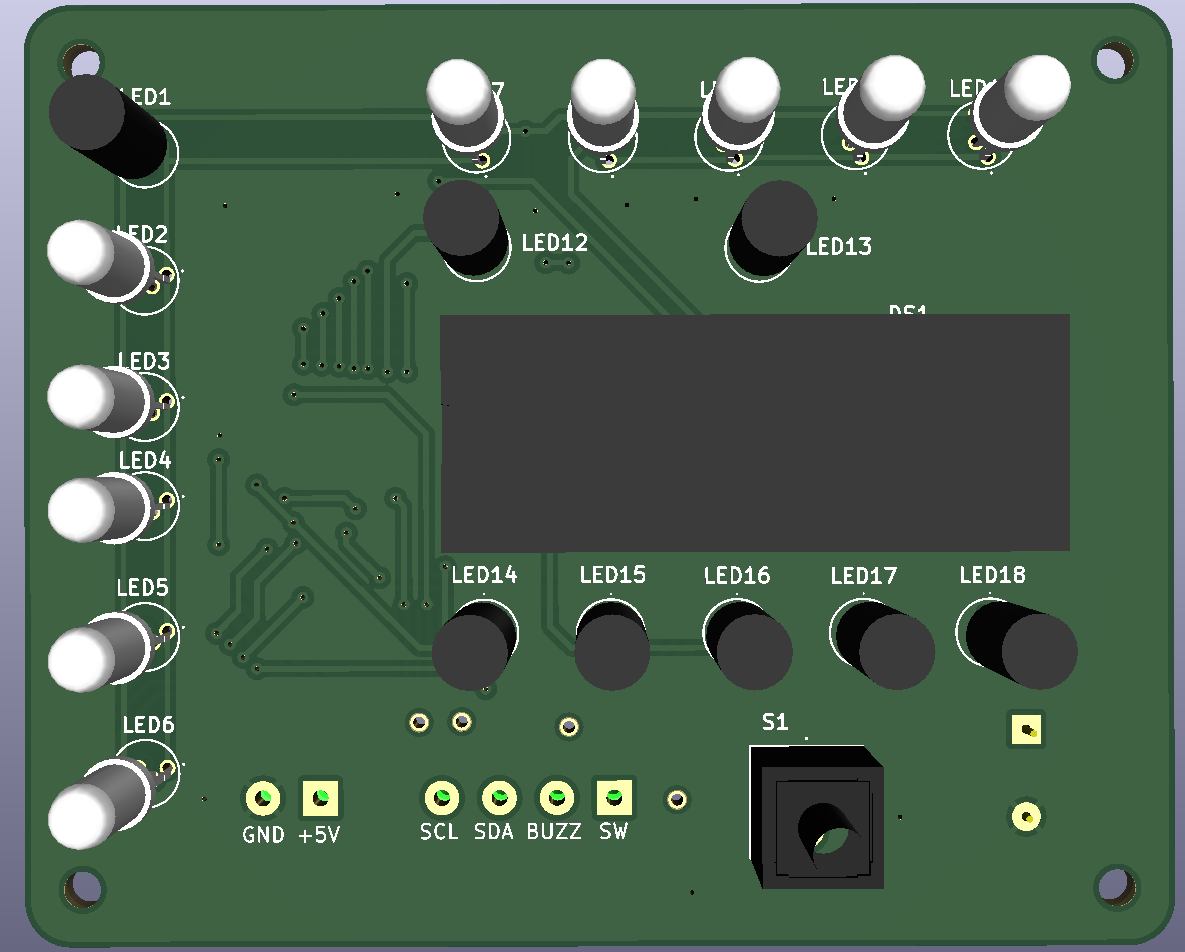
\includegraphics[width = 0.49\linewidth]{img/pcb_ihm_3d.png}
    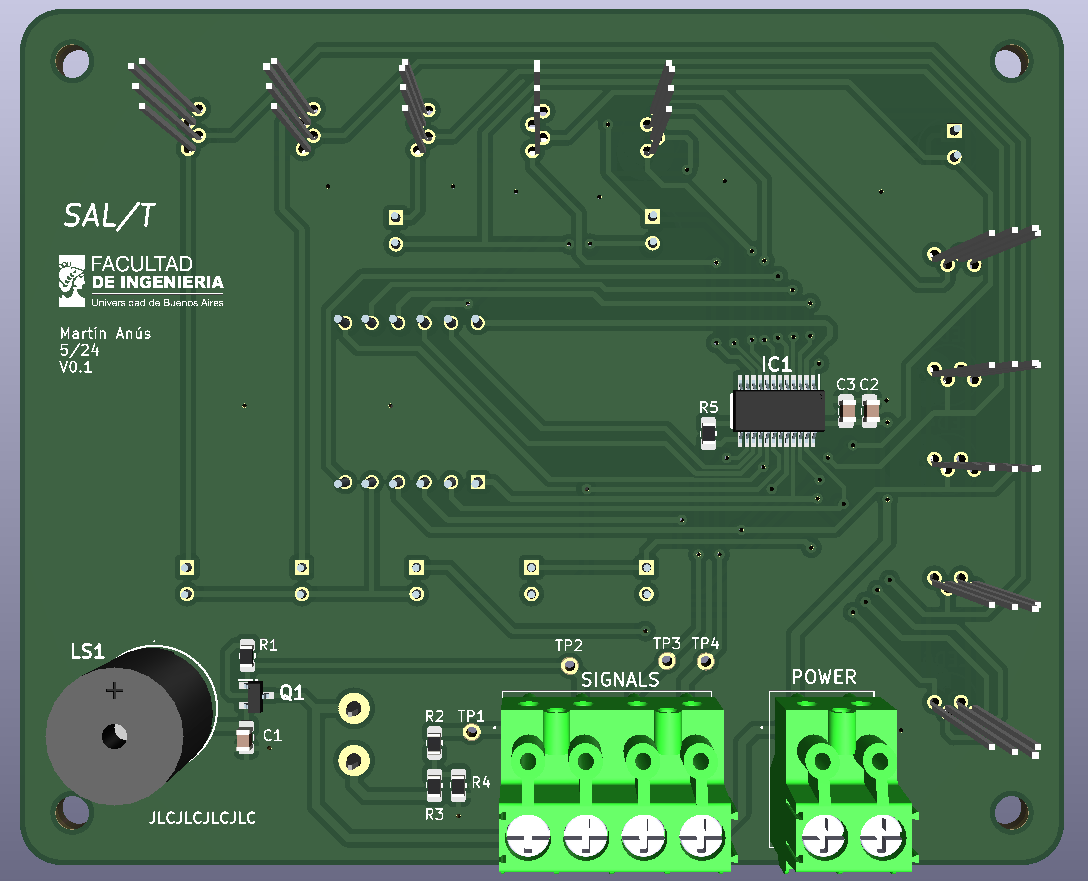
\includegraphics[width = 0.49\linewidth]{img/pcb_ihm_back_3d.png}
    \caption{Modelo 3D de la placa secundaria del SAL/T}
    \label{fig:salt_ihm_3d}
\end{figure}    




Los componentes fueron soldados a mano utilizando soldaduras de estaño. En las figuras \ref{fig:pcb_salt} y \ref{fig:pcb_salt_ihm} se visualiza la placa principal y la placa secundaria armada con todos los componentes montados. 

\begin{figure}[H]
    \centering
    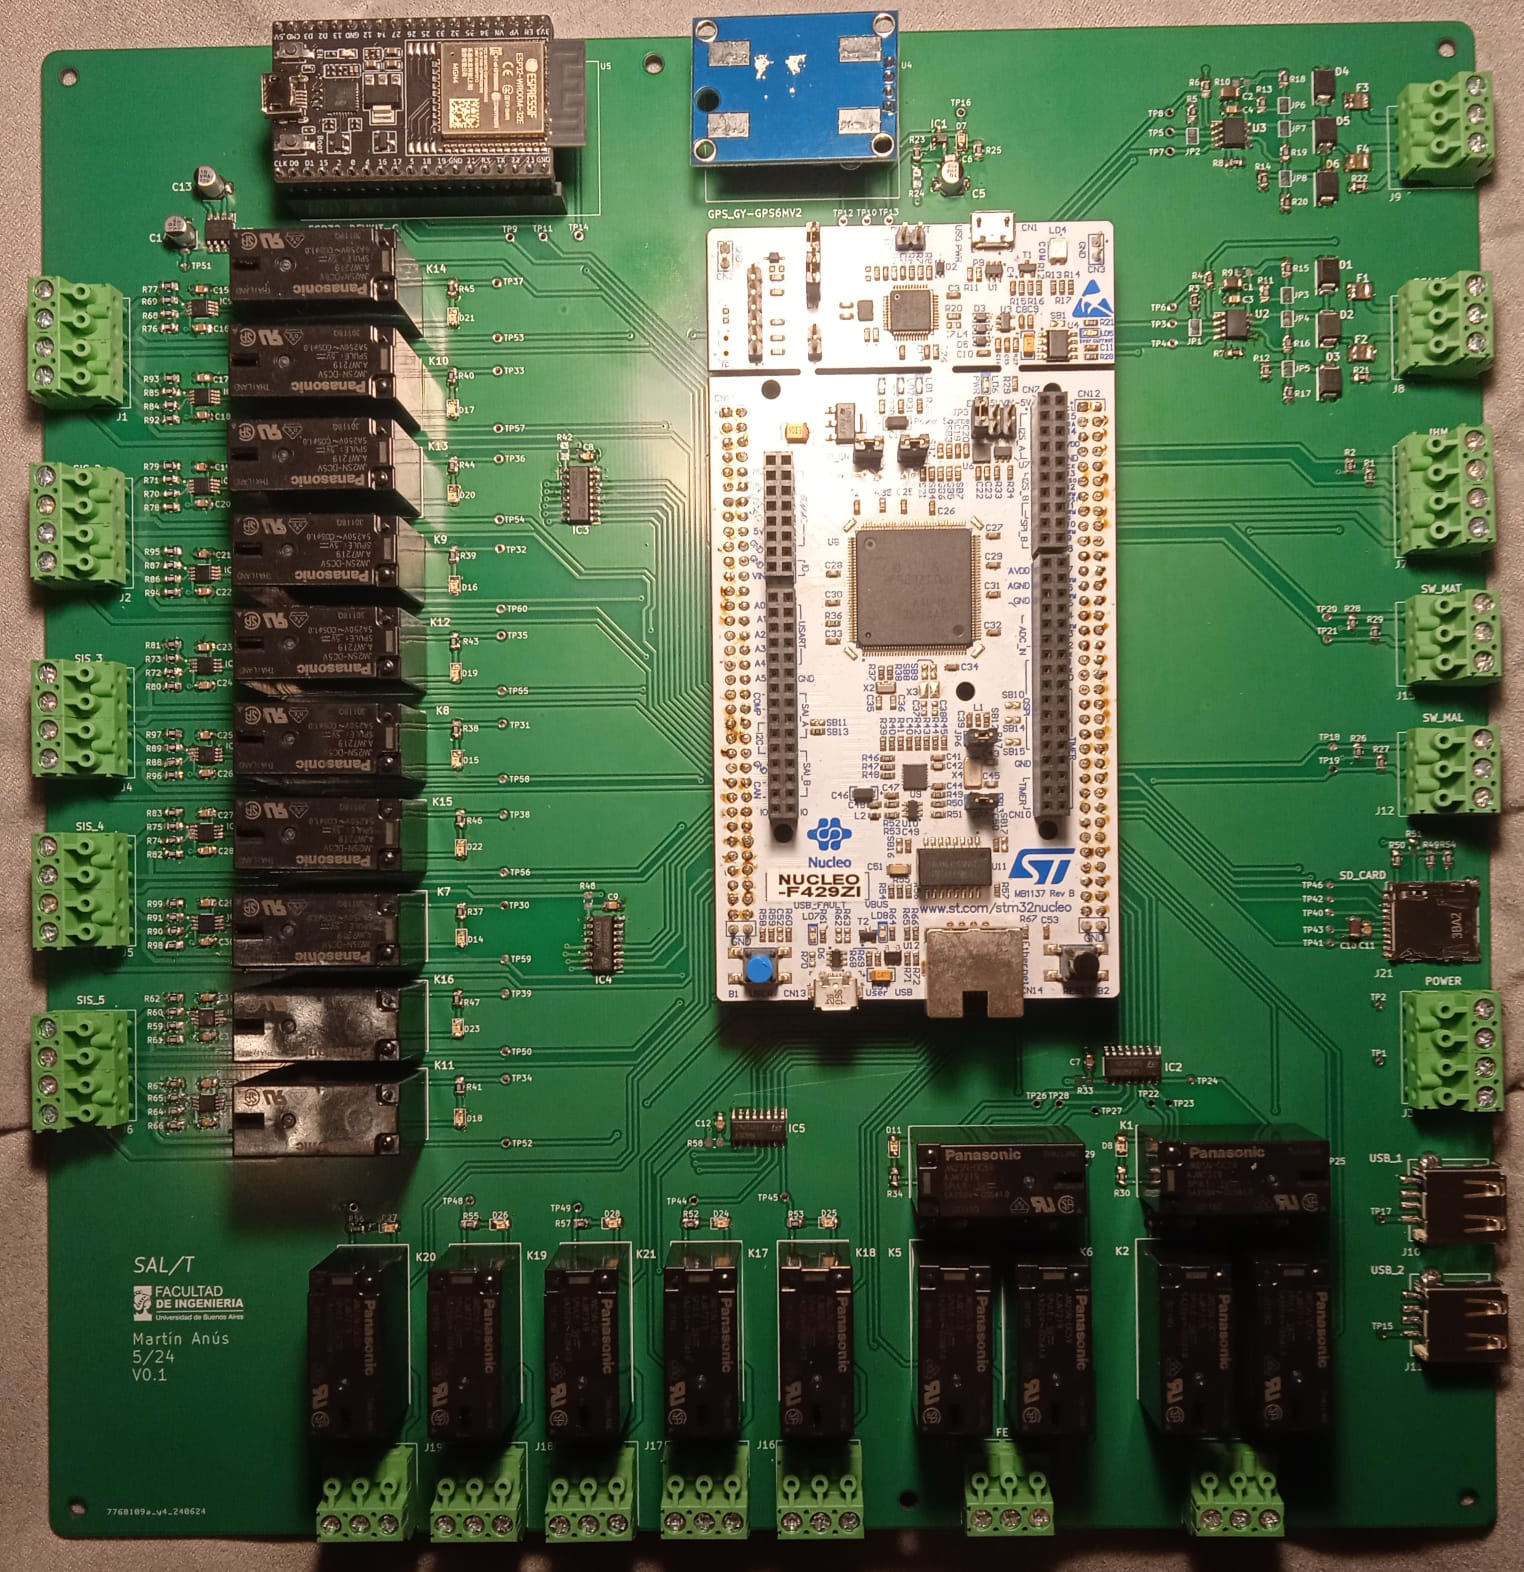
\includegraphics[width = \linewidth]{img/salt-placa_principal.jpeg}
    \caption{Placa principal del SAL/T fabricada}
    \label{fig:pcb_salt}
\end{figure}    



\begin{figure}[H]
    \centering
    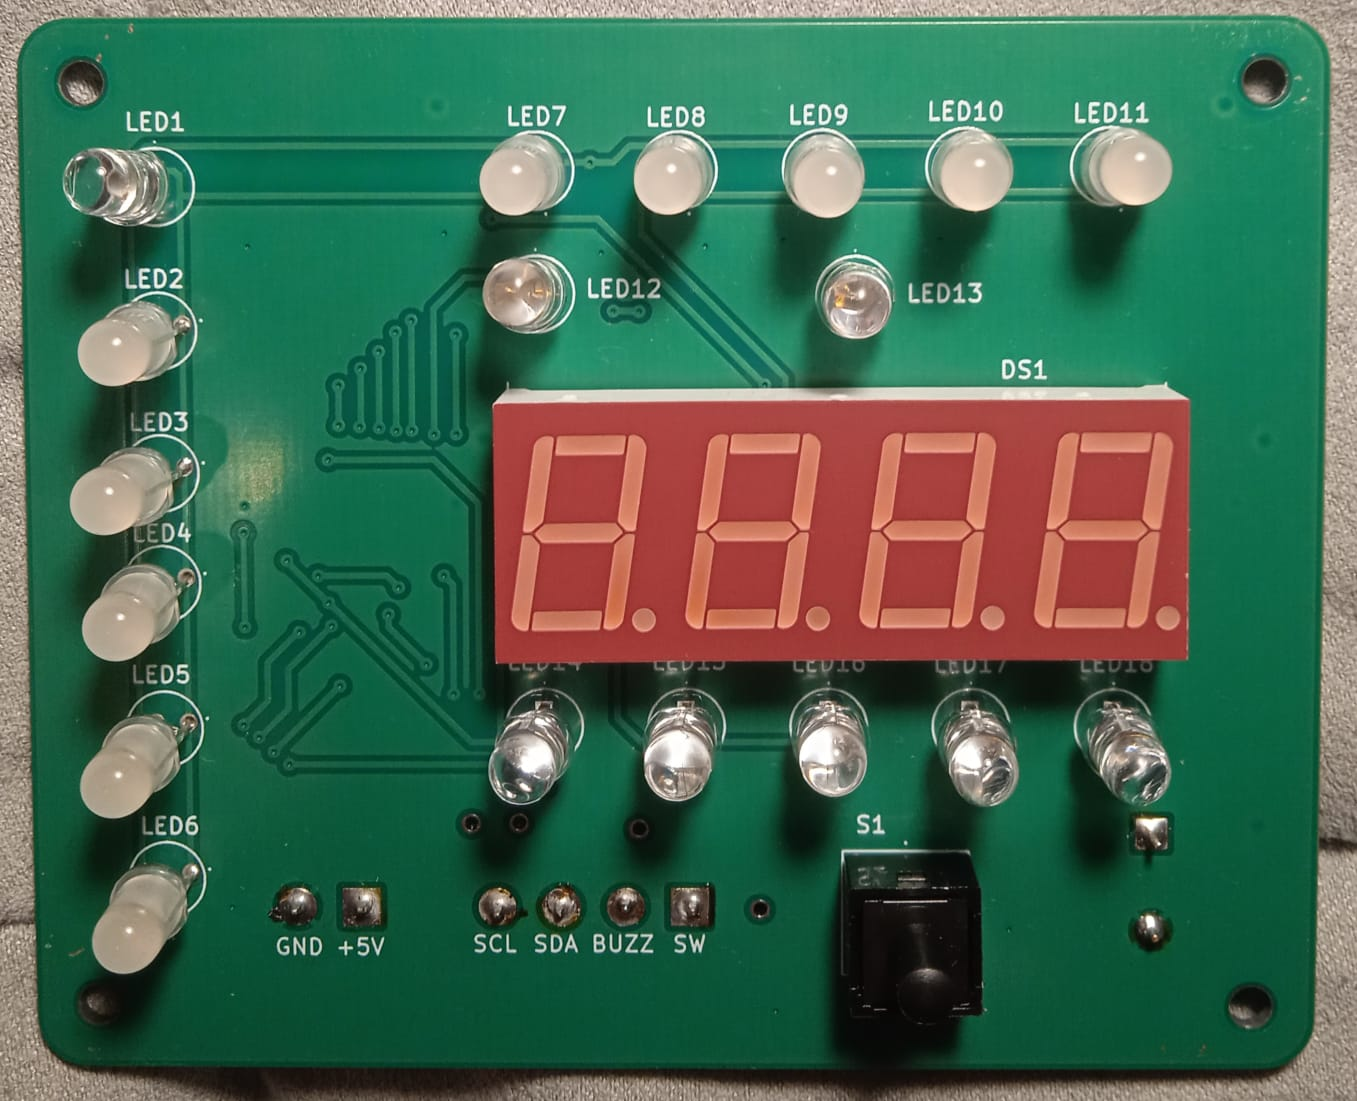
\includegraphics[width = 0.49\linewidth]{img/salt-placa_secundaria-front.jpeg}
    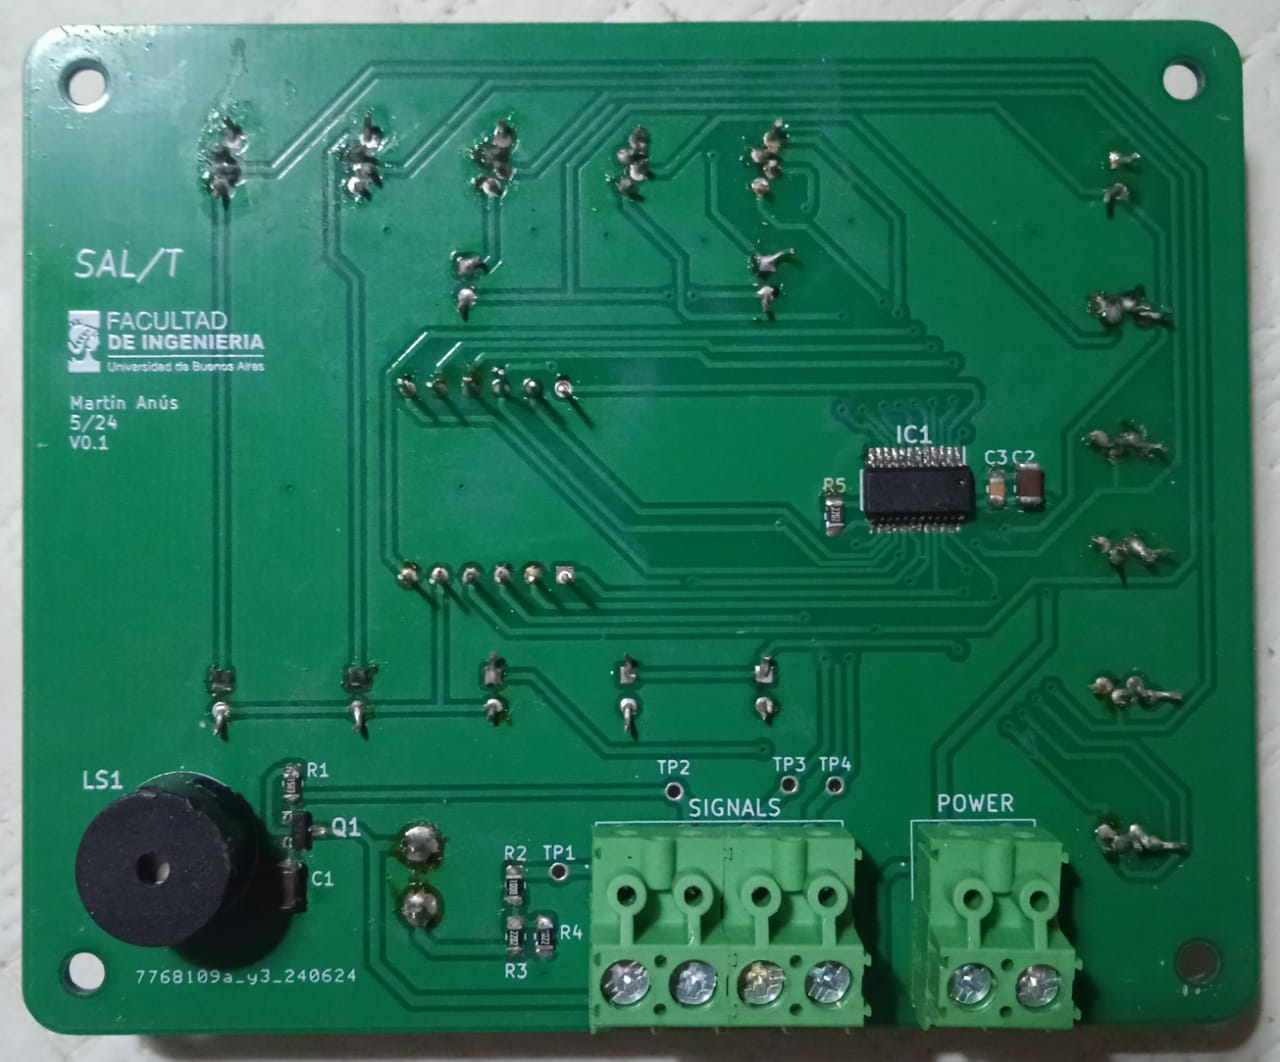
\includegraphics[width = 0.49\linewidth]{img/salt-placa_secundaria-back.jpeg}
    \caption{Placa secundaria del SAL/T fabricada}
    \label{fig:pcb_salt_ihm}
\end{figure}    